\documentclass{article}

\usepackage{arxiv}

\usepackage[utf8]{inputenc} % allow utf-8 input
\usepackage[T1]{fontenc}    % use 8-bit T1 fonts
\usepackage{hyperref}       % hyperlinks
\usepackage{url}            % simple URL typesetting
\usepackage{booktabs}       % professional-quality tables
\usepackage{amsfonts}       % blackboard math symbols
\usepackage{amsmath}
\usepackage{nicefrac}       % compact symbols for 1/2, etc.
\usepackage{microtype}      % microtypography
\usepackage{graphicx}
\usepackage{natbib}
\usepackage{doi}
\usepackage{csquotes}


\def \thetitle {Correcting supernova luminosity for redshift implies no accelerated expansion}
\title{\thetitle}

\date{\today}

\author{
  \href{https://orcid.org/0000-0001-6450-3262}{
\includegraphics[scale=0.06]{orcid.pdf}\hspace{1mm}Logan P.~Evans}
  \\ \texttt{loganpevans@gmail.com}
}

% Uncomment to override  the `A preprint' in the header
%\renewcommand{\headeright}{Technical Report}
%\renewcommand{\undertitle}{Technical Report}
\renewcommand{\shorttitle}{\textit{arXiv} Template}

%%% Add PDF metadata to help others organize their library
%%% Once the PDF is generated, you can check the metadata with
%%% $ pdfinfo template.pdf
\hypersetup{
pdftitle={\thetitle},
pdfsubject={astro-ph.CO},
pdfauthor={Logan P.~Evans},
pdfkeywords={cosmological parameters, dark energy},
}

\newtheorem{theorem}{Theorem}
\newtheorem{corollary}{Corollary}
\newtheorem{lemma}{Lemma}

\begin{document}
\maketitle

\begin{abstract}
  Existing analysis of Type Ia supernova relies on the assumption that
  luminosity is not affected by redshift. However, when luminosity is corrected
  for redshift, the relationship between luminosity distance and redshift for
  Type Ia supernova becomes linear. This implies that the expansion rate of the
  universe is not accelerating and there is no need for dark energy to explain
  observational data.
\end{abstract}

% keywords can be removed
\keywords{Cosmological Parameters \and Dark Energy \and Luminosity Distance}

\section{Introduction}

TODO: Discuss \citet{riess1998}, \citet{perlmutter1999}, and \citet{perlmutter2003}, as well as their nobel prize, summarized in \citet{straumann2012}.

Summarize dark energy. Emphasize that dark energy is a popular explanation for
why distant supernova appear to be too far away.

Talk about the difficulty of curating supernova data, and summarize the work
done by \citet{betoule2014}.

\begin{displayquote}
\end{displayquote}

\section{Derivation of luminosity distance}

Luminosity distance $D_L$, is the apparent distance of an object based on the
observed luminisity, also known as the flux $F$.  This does not take into
account any movement of the observed object between the time when the light was
emitted and the light is observed. $D_L$ also does not take into account
redshift. We are instead interested in $D_{L^*}$, which is the distance based
on the luminosity corrected for redshift.

Measurements of Type Ia supernova provide magnitude and redshift. To derive the
luminosity distance from these measurements, we start by computing the flux
$L$. Magnitude $M$ is defined on a logarithmic scale where magnitude 1 has 100
times the brightness of magnitude 6, leading to

\begin{equation}
  F = \frac{1}{\sqrt[5]{100}^{M - 1}}.
\end{equation}

This is proportional to the amount of energy detected by a telescope. However,
we instead want a number that is proportional to the number of photons detected
by the telescope. Redshifting decreases the amount of energy carried by a
photon from $E_{\text{emit}}$ to $E_{\text{obs}}$, but we can correct for this
phenomenon by taking

\begin{equation}
  F^{*} = F \frac{E_{\text{emit}}}{E_{\text{obs}}}.
\end{equation}

Since the energy for a photon is given by $E = \frac{hc}{\lambda}$ where $h$ is
the Planck constant and $c$ is the speed of light, we have

\begin{equation}
\begin{aligned}
  F^{*} &= F \frac{\frac{hc}{\lambda_{\text{emit}}}}{\frac{hc}{\lambda_{\text{obs}}}} \\
        &= F \frac{\lambda_{\text{obs}}}{\lambda_{\text{emit}}}.
\end{aligned}
\end{equation}

We use the redshift equation $(1 + z)\lambda_{\text{emit}} =
\lambda_{\text{obs}}$ to obtain

\begin{equation}
\begin{aligned}
  F^{*} &= B \frac{(1 + z)\lambda_{\text{emit}}}{\lambda_{\text{emit}}} \\
        &= B(1 + z).
\end{aligned}
\end{equation}

To compute the corrected magnitue $M^*$, we can solve

\begin{equation}
\begin{aligned}
   F^* &= \frac{1}{\sqrt[5]{100}^{M^* - 1}} \\
   M^* &= M - \frac{\ln{(z + 1)}}{\ln{(\sqrt[5]{100})}}.
\end{aligned}
\end{equation}

We note that since all Type Ia supernova have approximately the same intrinsic
brightness, we can use a geometric model to compute relative distances. Imagine
holding up two coins, one in each hand.  If you arange them so that the
distance from your eyes to the first coin double the distance from your eyes to
the second coin, the second coin should appear to be $\frac{1}{4}$ of the size.
More formally, for two objects of the same radius $r$, the apparent area $A$
is

\begin{equation}
  A = \pi \bigg(\frac{r}{d}\bigg)^2
\end{equation}

where $D$ is the relative distance between the two objects.

Replacing the area with the brightness, we have

\begin{equation*}
  F^{*} = \pi \bigg(\frac{r}{D}\bigg)^2
\end{equation*}

\begin{equation}
\label{eq:D*}
  D_{L^*} = r \sqrt{\frac{\pi}{F^*}}.
\end{equation}

Since this equation has no specified units, we will need to find a
calibration factor $k$. To beautify the equation, we can collect all constants
(which includes $r$ since all Type Ia supernova have the same intrinsic
brightness) into $k$. This gives

\begin{equation}
\begin{aligned}
  D_{L^*} &= r \sqrt{\frac{\pi}{\frac{1}{\sqrt[5]{100}^{M - 1}}(1 + z)}} \\
          &= \frac{k 10^\frac{M}{5}}{\sqrt{z + 1}}.
\end{aligned}
\end{equation}

The results of this model are shown in Figure \ref{fig:corrected_uncalibrated}.

\begin{figure}[h!]
  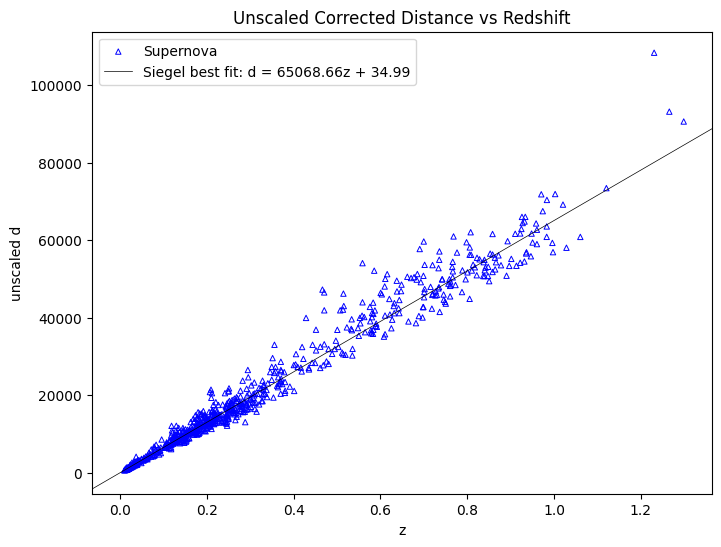
\includegraphics[width=\linewidth]{../graphs/corrected_uncalibrated.png}
  \caption{Uncalibrated distance model using the corrected $F^*$ values for
  brightness. The data were obtained from \citet{betoule2014}.}
  \label{fig:corrected_uncalibrated}
\end{figure}

\begin{figure}[h!]
  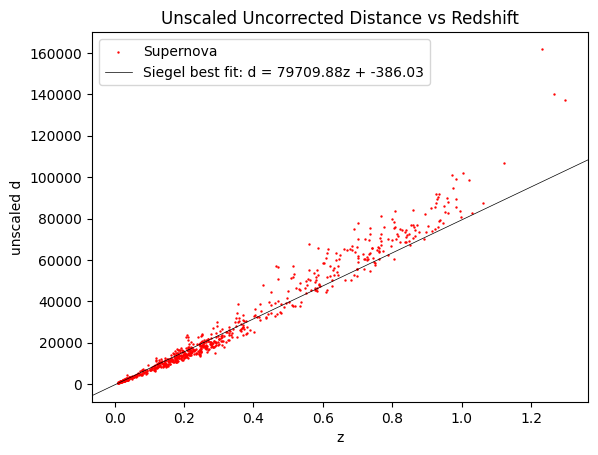
\includegraphics[width=\linewidth]{../graphs/uncorrected_uncalibrated.png}
  \caption{Uncalibrated distance model using the uncorrected $F$ values for brightness.
  The deviation from linearity suggests that distant objects are
  farther away than expected due to an accelerated expansion rate.}
  \label{fig:uncorrected_uncalibrated}
\end{figure}

\section{Calibrated distance models}
\label{sec:calibrated}

Calibrating a distance model involves finding a linear regression line for a
model and then computing the value $k$ required to make the regression model
match a Hubble paramater. By arbitrary choice, we use $H_0 = 70 \frac{km/s}{Mpsc}$.

The final units for distance will be in megaparsecs $Mpsc$. To find the
recessional speed for a given redshift, we use $v = cz$ where $c$ is the speed
of light.

To compute a model, we use non-parametric regression via repeated means as described in
\citet{siegel1982}. A comparison of both models is shown in Figure \ref{fig:calibrated}.

\begin{figure}[h!]
  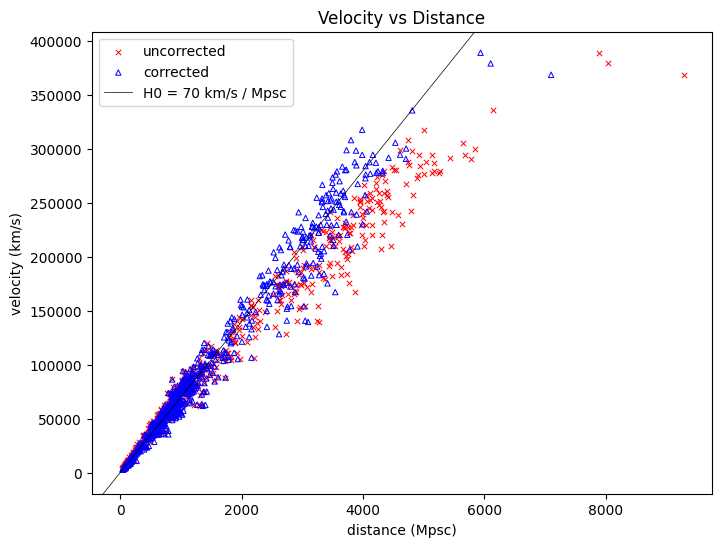
\includegraphics[width=\linewidth]{../graphs/both_calibrated_velocity_vs_distance.png}
  \caption{Calibrated distance model using both the corrected $F^*$ values as
  well as the uncorrected $F$ brightness values.}
  \label{fig:calibrated}
\end{figure}

\section{Disagreement with existing research}

Previous studies use $F$ instead of $F*$. According to \citet{betoule2014},

\begin{displayquote}
  Specifically, the distance estimator used in this analysis (and in most
  similar cosmological analyses) assumes that supernovae with identical color,
  shape and galactic environment have on average the same intrinsic luminosity
  for all redshifts. This hypothesis is quantified by a linear model, yielding
  a standardized distance modulus $\mu = 5 \log_{10}{(d_L / 10 \text{pc})}$:

  \begin{equation}
  \label{eq:betoule_distance_modulus}
    \mu = m_B^* - (M_B - \alpha \times X_1 + \beta \times C)
  \end{equation}

  where $m_B^*$ corresponds to the observed peak magnitude in restframe $B$
  band and $\alpha$, $\beta$ and $M_B$ are nuisance parameters in the distance
  estimate.
\end{displayquote}

This statement may refer to the idea that a Type Ia supernova can have an
evolving intrinsic luminosity $L$ over time as conditions within the universe
change which was first hypothesized by \citet{tinsley1968}. In Equation
\ref{eq:betoule_distance_modulus}, there is no correction for redshift, which
suggests the interpretation that the flux $F$ is unaffected by redshift.

The model where $F$ is not corrected for redshift is explored in Figure
\ref{fig_uncorrected_uncalibrated} by replacing $F^*$ with $F$ in Equation
\ref{eq:D*} and obtaining

\begin{equation}
  D_L = k 10^\frac{M}{5}.
\end{equation}

\section{Conclusions}
\label{sec:conclusions}

\bibliographystyle{unsrtnat}
\bibliography{references}

\end{document}
